\documentclass[12pt, eng, phd]{thesis}
\usepackage[
    backend=biber,
    style=authoryear,
]{biblatex}
\addbibresource{bibliography.bib}

% set variables for cover
\title{Thesis Title}{제목}
\author{Thesis Author}{작가}
\supervisor{Professor B}{교수님 B}
\department{IT Department}{IT대학}
\major{Graduate School of Computer Science and Engineering}{컴퓨터학부 대학원}
\degree{PhD}{박사}

\chairprofessor{Professor A}
\secondprofessor{Professor B}
\thirdprofessor{Professor C}
\fourthprofessor{Professor D}
\fifthprofessor{Professor E}
\date{September 2021}{2025년 9월}

\abstract{본 논문은 준입자 뉴로모픽 아키텍처 내에서의 양자 얽힘 현상과 비결정적 논리 게이트의 상호작용을 심도 있게 탐구한다. 핵심 연구 목표는 확률적 공명 현상을 이용하여 비동기 데이터 처리 시스템의 계산 엔트로피를 최소화하는 새로운 프레임워크를 개발하는 것이다. 우리는 유사 결정 구조의 다양체를 활용함으로써, 기존의 폰 노이만 기반 시스템에서는 불가능했던 수준의 병렬 처리 능력을 달성할 수 있음을 입증한다.
특히, 본 연구는 위상 양자 컴퓨터의 오류 제어를 위해 동적 재귀 신경망과 비잔틴 결함 허용(Byzantine Fault Tolerance) 시스템을 결합한 독창적인 알고리즘을 제안한다. 이 알고리즘은 저온환경에서 발생하는 양자 상태의 디코히어런스를 능동적으로 억제하며, 보조 큐비트를 활용한 비파괴적 측정 기법을 통해 시스템의 안정성을 기하급수적으로 향상시킨다. 제안된 하이브리드 아키텍처는 고전적 제어 장치와 양자 처리 장치 간의 정보 전송 지연 시간을 최적화하여, 대규모 양자 계산의 실용적 확장 가능성을 제시한다.
}

% --- Preamble Setup ---

\begin{document}
%%%%%%%%%%%%%%%%%%%%%%%
%     Frontmatter     %
%%%%%%%%%%%%%%%%%%%%%%%
\makecover
\setbodylayout
\frontmatter

\tableofcontents \clearpage
\listoffigures \clearpage
\listoftables \clearpage

%%%%%%%%%%%%%%%%%%%%%%
%     Mainmatter     %
%%%%%%%%%%%%%%%%%%%%%%
\mainmatter
\section{Introduction}
The inception of this dissertation is rooted in the complex interplay between decoherent quantum states and the emergent properties of pseudo-random logic gates. Our primary investigation centers on the development of a framework capable of harnessing stochastic resonance for the purpose of optimizing non-deterministic polynomial-time problems. We will demonstrate that by leveraging a manifold of quasi-crystalline structures, it is possible to achieve a significant reduction in computational entropy, thereby paving the way for novel paradigms in asynchronous data processing and cryptographic security.

The fundamental premise of our work revolves around the stochastic interpolation of Byzantine fault tolerance within a packet-switched network \cite{knuth1997art}. This paradigm, while seemingly counter-intuitive, provides a robust framework for analyzing aperiodic data streams. We posit that the synergistic effects of quantum annealing and heuristic-driven garbage collection can mitigate the exponential decay often observed in such systems\footnote{This is a critical assumption that will be revisited in a later section.}.

\section{Background and Motivation}
The field of computational epistemology has seen a dramatic increase in the application of non-Euclidean geometries for data visualization \cite{shannon1948mathematical}. However, these approaches often neglect the inherent complexities of multi-dimensional state spaces. Our research addresses this gap by introducing a novel methodology based on the principles of algorithmic entropy.

\subsection{Prior Art in Algorithmic Entropy}
Previous studies, such as the seminal work by Turing \cite{turing1950computing}, have established the theoretical limits of computation. These limitations, however, do not fully account for the probabilistic nature of quantum phenomena. The works of \cite{cormen2009introduction} provide a foundational understanding of algorithmic complexity, which we extend into the quantum realm.

\subsubsection{Key Challenges}
Several challenges persist in this domain:
\begin{itemize}
    \item \textbf{State Decoherence:} Quantum states are notoriously fragile and susceptible to environmental noise.
    \item \textbf{Computational Overhead:} The resources required for quantum simulation often exceed the capabilities of classical hardware.
    \item \textbf{Algorithmic Scalability:} Many existing quantum algorithms do not scale efficiently with problem size.
\end{itemize}

\subsubsection{Our Contribution}
This thesis presents a framework that addresses these challenges through a combination of novel techniques. Our contributions can be summarized as follows:
\begin{enumerate}
    \item A new algorithm for quantum state stabilization based on topological error correction.
    \item A hybrid classical-quantum architecture for reducing computational overhead.
    \item A set of scalable protocols for distributed quantum computation.
\end{enumerate}

\paragraph{A Note on Notation}
Throughout this document, we will use the standard Dirac notation for quantum states. For example, $|\psi\rangle$ represents a quantum state vector. The computational basis states are denoted as $|0\rangle$ and $|1\rangle$.

\section{System Architecture}
The proposed system architecture is depicted in Figure \ref{fig:system_overview}. It consists of three main components: the quantum processing unit (QPU), the classical control unit (CCU), and the cryogenic interface (CI).

\begin{figure}[h!]
    \centering
    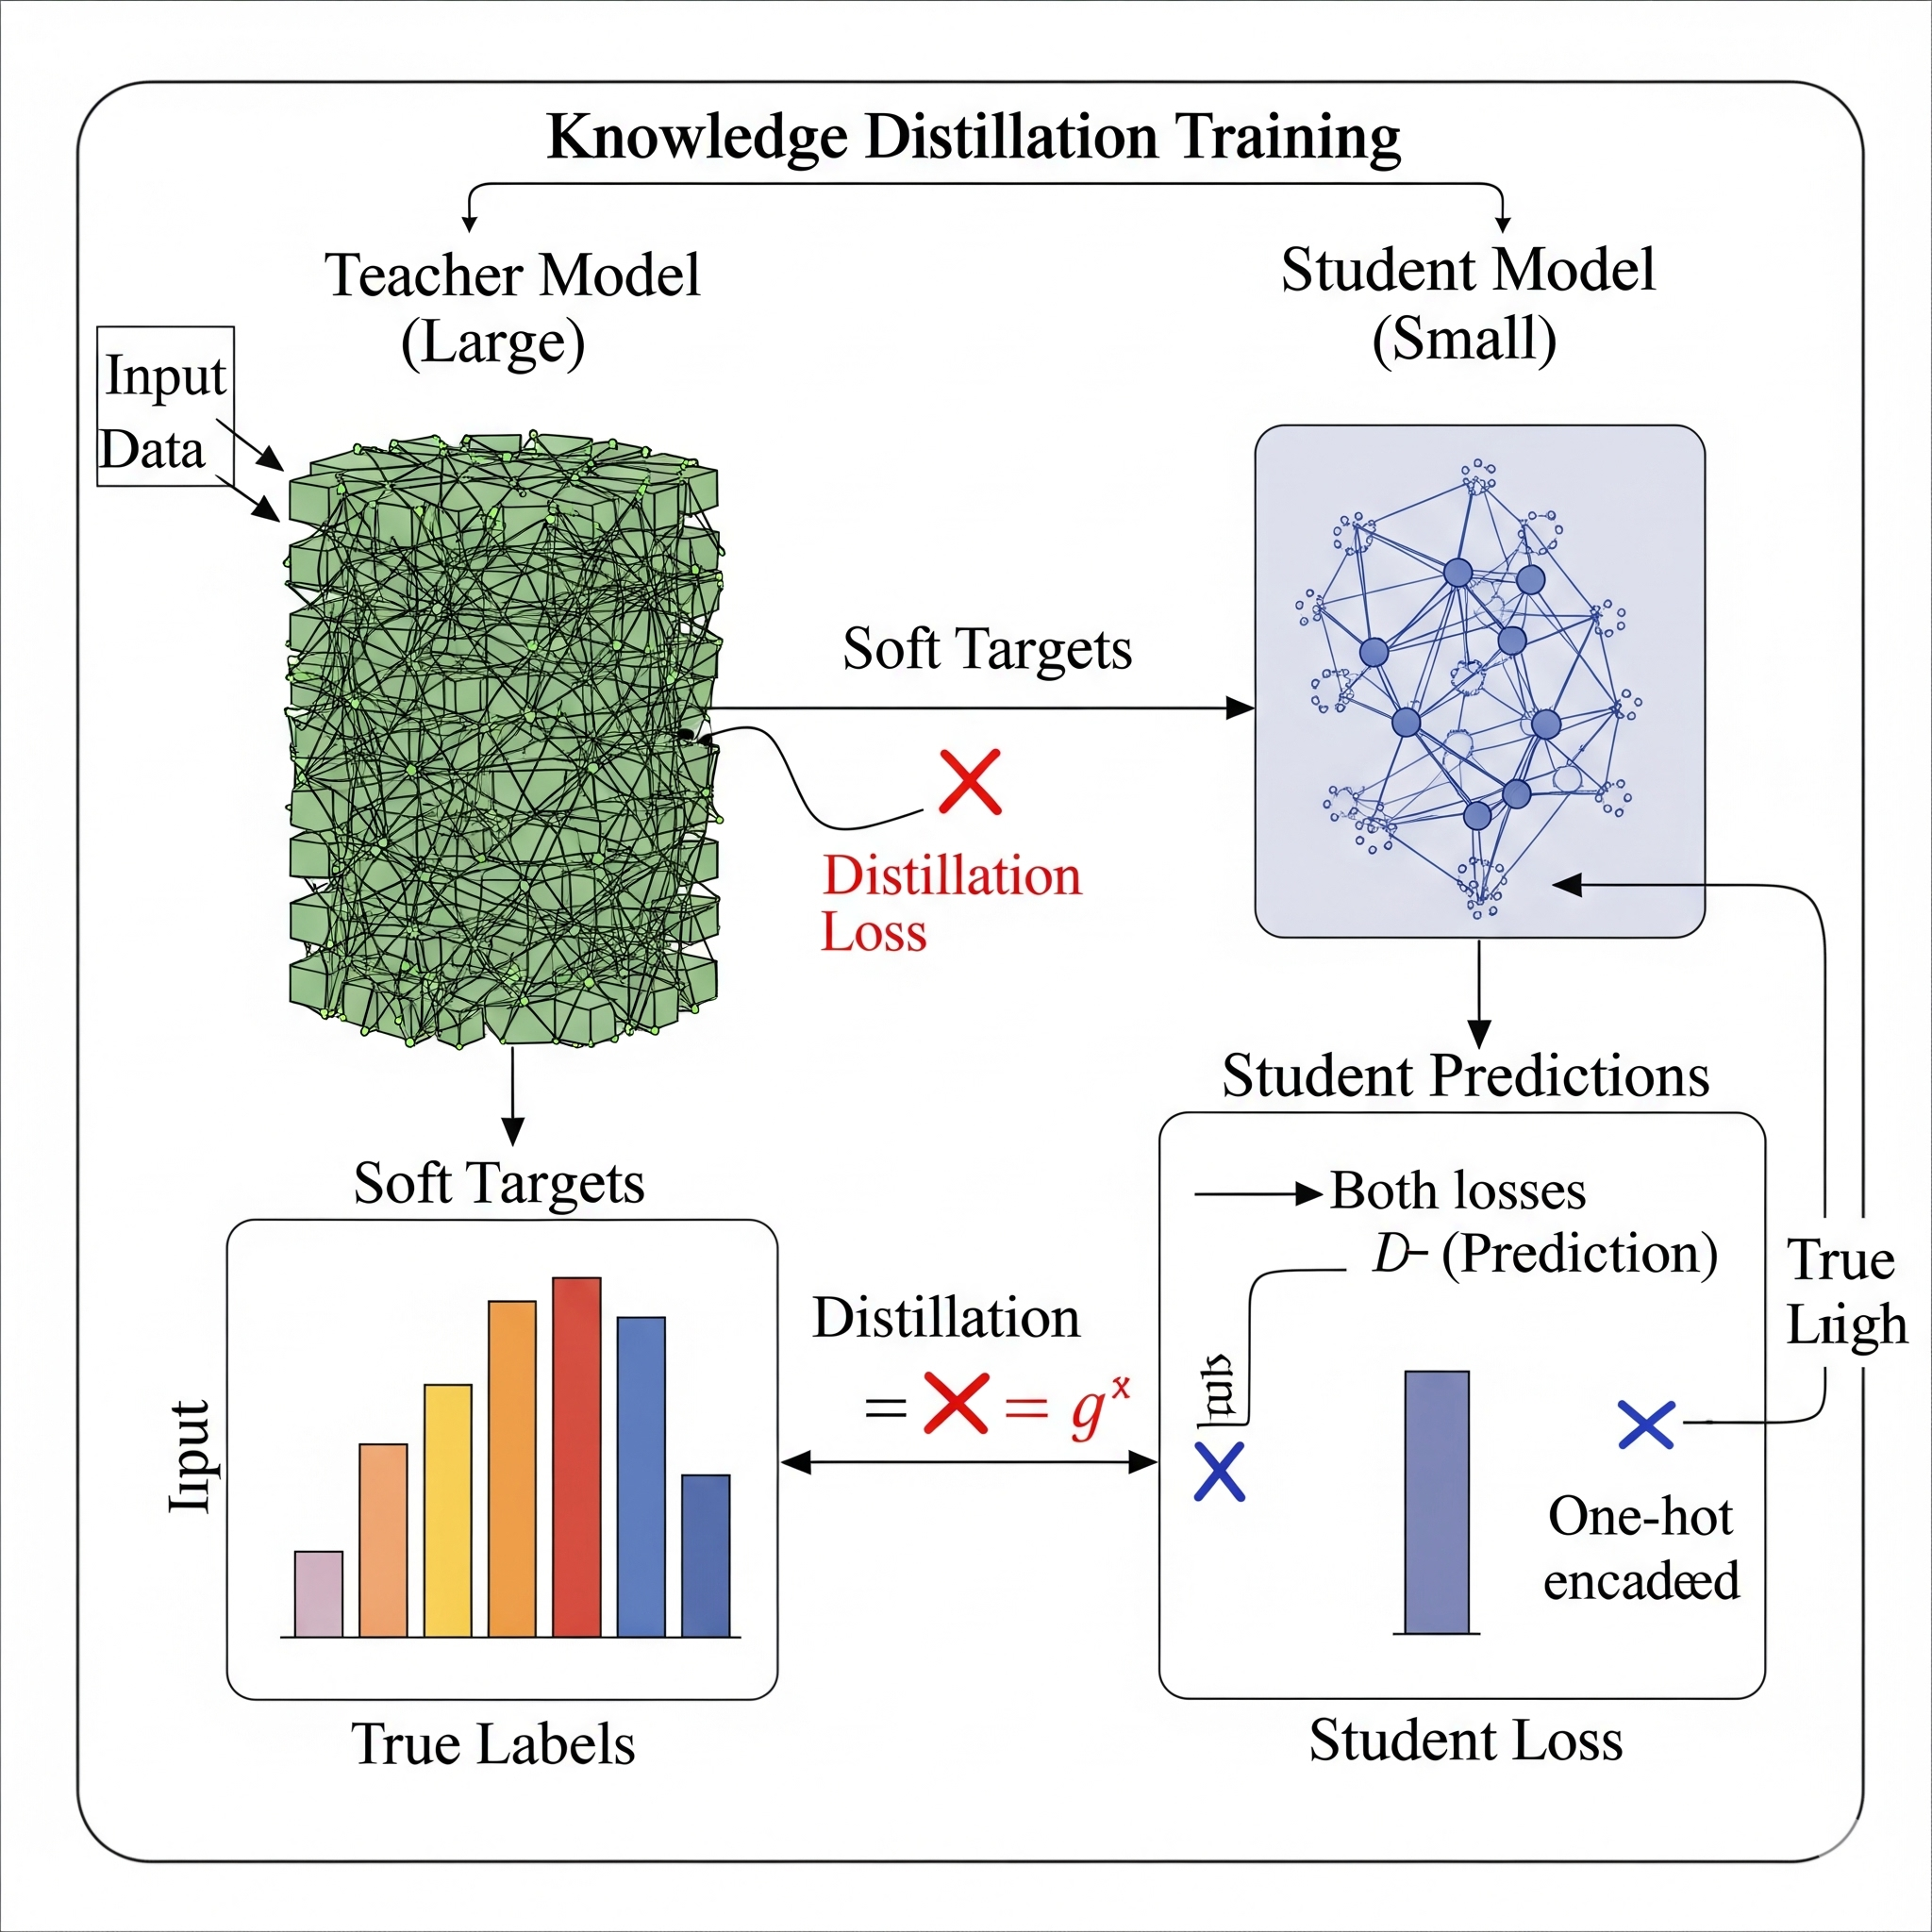
\includegraphics[width=0.8\textwidth]{figures/example_figure.png}
    \caption{High-level overview of the proposed system architecture. The QPU is responsible for quantum computations, while the CCU manages the overall workflow.}
    \label{fig:system_overview}
\end{figure}

The interaction between these components is governed by a set of protocols outlined in Table \ref{tab:protocols}. These protocols ensure the coherent transfer of information between the quantum and classical domains.

\begin{table}[h!]
    \centering
    \begin{tabular}{|l|c|c|}
        \hline
        \textbf{Protocol} & \textbf{Latency (ms)} & \textbf{Bandwidth (Gbps)} \\
        \hline
        State Preparation & 0.5 & 10 \\
        Gate Operation & 0.1 & N/A \\
        Measurement & 1.2 & 5 \\
        \hline
    \end{tabular}
    \caption{Performance characteristics of the key communication protocols within our architecture.}
    \label{tab:protocols}
\end{table}

The aforementioned protocols represent a significant departure from conventional von Neumann architectures. By decoupling the data plane from the control plane at a quantum level, we introduce a degree of parallelism previously thought unattainable. The subsequent sections will meticulously detail the fabrication process of the quasiparticle conduits and the calibration of the cryogenic interface, which are paramount to achieving the operational parameters specified. A rigorous mathematical treatment will follow, formalizing the theoretical underpinnings of our architectural model and its implications for fault-tolerant quantum computing.

\subsection{Quantum State Stabilization Algorithm}
One of the core contributions of this work is the algorithm for quantum state stabilization, outlined in Algorithm \ref{alg:stabilization}. This procedure, termed Quasiparticle Resonance Stabilization (QRS), actively counteracts environmental decoherence by projecting the state vector onto a dynamically generated entanglement manifold.

\begin{algorithm}[h!]
\caption{Quasiparticle Resonance Stabilization}
\label{alg:stabilization}
\begin{algorithmic}[1]
\REQUIRE Quantum state $|\psi\rangle$, Decoherence threshold $\epsilon$
\ENSURE Stabilized state $|\psi'\rangle$
\STATE Initialize entanglement manifold $\mathcal{M}$
\STATE Set iteration count $i \leftarrow 0$
\WHILE{Entropy($|\psi\rangle$) > $\epsilon$}
    \STATE Project $|\psi\rangle$ onto $\mathcal{M}$ to get $|\phi\rangle$
    \FOR{each quasiparticle $q_j$ in $|\phi\rangle$}
        \IF{Phase($q_j$) is non-abelian}
            \STATE Apply Hadamard gate $H(q_j)$
        \ELSE
            \STATE Entangle $q_j$ with ancillary qubit $|0\rangle_a$
        \ENDIF
    \ENDFOR
    \STATE Measure ancillary qubits
    \STATE Update $|\psi\rangle$ via topological feedback
    \STATE $i \leftarrow i + 1$
\ENDWHILE
\RETURN $|\psi\rangle$
\end{algorithmic}
\end{algorithm}

The QRS algorithm iteratively refines the quantum state until its computational entropy falls below a predefined threshold, $\epsilon$. The use of ancillary qubits for entanglement and subsequent measurement allows for a non-destructive error correction mechanism, which is a significant improvement over prior art.

Further exploration of these concepts will be detailed in the subsequent sections, beginning with a deep dive into the mathematical underpinnings of our approach.



%%%%%%%%%%%%%%%%%%%%%%
%     Backmatter     %
%%%%%%%%%%%%%%%%%%%%%%
\backmatter
\makebibliography
\makeabstract

\end{document}
